%% abtex2-modelo-relatorio-tecnico.tex, v-1.7.1 laurocesar
%% Copyright 2012-2013 by abnTeX2 group at http://abntex2.googlecode.com/ 
%%
%% This work may be distributed and/or modified under the
%% conditions of the LaTeX Project Public License, either version 1.3
%% of this license or (at your option) any later version.
%% The latest version of this license is in
%%   http://www.latex-project.org/lppl.txt
%% and version 1.3 or later is part of all distributions of LaTeX
%% version 2005/12/01 or later.
%%
%% This work has the LPPL maintenance status `maintained'.
%% 
%% The Current Maintainer of this work is the abnTeX2 team, led
%% by Lauro César Araujo. Further information are available on 
%% http://abntex2.googlecode.com/
%%
%% This work consists of the files abntex2-modelo-relatorio-tecnico.tex,
%% abntex2-modelo-include-comandos and abntex2-modelo-references.bib
%%

% ------------------------------------------------------------------------
% ------------------------------------------------------------------------
% abnTeX2: Modelo de Relatório Técnico/Acadêmico em conformidade com 
% ABNT NBR 10719:2011 Informação e documentação - Relatório técnico e/ou
% científico - Apresentação
% ------------------------------------------------------------------------ 
% ------------------------------------------------------------------------

% Alterado por Rodrigo Campiolo para apresentação de relatórios na disciplina
% de Redes de Computadores II do Bacharelado em Ciência da Computação da UTFPR-CM.


\documentclass[
    % -- opções da classe memoir --
    12pt,				% tamanho da fonte
    %openright,			% capítulos começam em pág ímpar (insere página vazia caso preciso)
    oneside,   	        % para impressão em verso e anverso use twoside. Oposto a oneside
    a4paper,			% tamanho do papel. 
    % -- opções da classe abntex2 --
    %chapter=TITLE,		% títulos de capítulos convertidos em letras maiúsculas
    %section=TITLE,		% títulos de seções convertidos em letras maiúsculas
    %subsection=TITLE,	% títulos de subseções convertidos em letras maiúsculas
    %subsubsection=TITLE,% títulos de subsubseções convertidos em letras maiúsculas
    % -- opções do pacote babel --
    english,			% idioma adicional para hifenização
    french,				% idioma adicional para hifenização
    spanish,			% idioma adicional para hifenização
    brazil,				% o último idioma é o principal do documento
    ]{pacotes/abntex2}


% ---
% PACOTES
% ---

% ---
% Pacotes fundamentais 
% ---
\usepackage{cmap}				% Mapear caracteres especiais no PDF
\usepackage{lmodern}			% Usa a fonte Latin Modern
\usepackage[T1]{fontenc}		% Selecao de codigos de fonte.
\usepackage[utf8]{inputenc}		% Codificacao do documento (conversão automática dos acentos)
\usepackage{indentfirst}		% Indenta o primeiro parágrafo de cada seção.
\usepackage{color}				% Controle das cores
\usepackage{graphicx}			% Inclusão de gráficos
% ---

% ---
% Pacotes adicionais, usados no anexo do modelo de folha de identificação
% ---
\usepackage{multicol}
\usepackage{multirow}
% ---
    
% ---
% Pacotes adicionais, usados apenas no âmbito do Modelo Canônico do abnteX2
% ---
\usepackage{lipsum}				% para geração de dummy text
% ---

% ---
% Pacotes de citações
% ---
\usepackage[brazilian,hyperpageref]{backref}	 % Paginas com as citações na bibl
\usepackage[alf]{pacotes/abntex2cite}	% Citações padrão ABNT
\usepackage{comment}
% ---

% ---
% Meus pacotes
% ---
\usepackage{float}
\usepackage{listings}
\usepackage{color}


\definecolor{codegreen}{rgb}{0,0.6,0}
\definecolor{codegray}{rgb}{0.5,0.5,0.5}
\definecolor{codepurple}{rgb}{0.58,0,0.82}
\definecolor{backcolour}{rgb}{0.95,0.95,0.92}

\lstdefinestyle{mystyle}{
  language=C++,
  backgroundcolor=\color{backcolour},   
  commentstyle=\color{codegreen},
  keywordstyle=\color{magenta},
  numberstyle=\tiny\color{codegray},
  stringstyle=\color{codepurple},
  basicstyle=\ttfamily\footnotesize,
  breakatwhitespace=false,         
  breaklines=true,                 
  captionpos=b,                    
  keepspaces=true,                 
  numbers=left,                    
  numbersep=5pt,                  
  showspaces=false,                
  showstringspaces=false,
  showtabs=false,                  
  tabsize=2
}

\lstset{style=mystyle}
% ---

% --- 
% CONFIGURAÇÕES DE PACOTES
% --- 

% ---
% Configurações do pacote backref
% Usado sem a opção hyperpageref de backref
\renewcommand{\backrefpagesname}{Citado na(s) página(s):~}
% Texto padrão antes do número das páginas
\renewcommand{\backref}{}
% Define os textos da citação
\renewcommand*{\backrefalt}[4]{
    \ifcase #1 %
        Nenhuma citação no texto.%
    \or
        Citado na página #2.%
    \else
        Citado #1 vezes nas páginas #2.%
    \fi}%
% ---

% ---
% Informações de dados para CAPA e FOLHA DE ROSTO
% ---
\titulo{Implementação do Sistema de Arquivos FAT32}
\autor{João Victor Briganti\\Luiz Gustavo Takeda\\Matheus Floriano Saito}
\local{Campo Mourão}
\data{Fevereiro / 2025}
\instituicao{%
  Universidade Tecnológica Federal do Paraná -- UTFPR
  \par
  Departa           mento Acadêmico de Computação -- DACOM
  \par
  Bacharelado em Ciência da Computação -- BCC
}
\tipotrabalho{Relatório técnico}
% O preambulo deve conter o tipo do trabalho, o objetivo, 
% o nome da instituição e a área de concentração 
\preambulo{Relatório técnico de atividade prática solicitado pelo professor Rodrigo Campiolo na disciplina de Sistemas Operacionais do Bacharelado em Ciência da Computação da Universidade Tecnológica Federal do Paraná.}
% ---

% ---
% Configurações de aparência do PDF final

% alterando o aspecto da cor azul
\definecolor{blue}{RGB}{41,5,195}

% informações do PDF
\makeatletter
\hypersetup{
        %pagebackref=true,
        pdftitle={\@title}, 
        pdfauthor={\@author},
        pdfsubject={\imprimirpreambulo},
        pdfcreator={LaTeX with abnTeX2},
        pdfkeywords={abnt}{latex}{abntex}{abntex2}{relatório técnico}, 
        colorlinks=true,       		% false: boxed links; true: colored links
        linkcolor=blue,          	% color of internal links
        citecolor=blue,        		% color of links to bibliography
        filecolor=magenta,      		% color of file links
        urlcolor=blue,
        bookmarksdepth=4
}
\makeatother
% --- 

% --- 
% Espaçamentos entre linhas e parágrafos 
% --- 

% O tamanho do parágrafo é dado por:
\setlength{\parindent}{1.3cm}

% Controle do espaçamento entre um parágrafo e outro:
\setlength{\parskip}{0.2cm}  % tente também \onelineskip

% ---
% compila o indice
% ---
\makeindex
% ---

% Omite a numeração de capítulos
\renewcommand*\thesection{\arabic{section}}



% ----
% Início do documento
% ----
\begin{document}

% Retira espaço extra obsoleto entre as frases.
\frenchspacing 

% ----------------------------------------------------------
% ELEMENTOS PRÉ-TEXTUAIS
% ----------------------------------------------------------
% \pretextual

% ---
% Capa
% ---
%\imprimircapa
% ---

% ---
% Folha de rosto
% (o * indica que haverá a ficha bibliográfica)
% ---
\imprimirfolhaderosto
% ---


% ---
% RESUMO
% ---

% resumo na língua vernácula (obrigatório)
\begin{resumo}

Este estudo teve como objetivo investigar e implementar um sistema de arquivos FAT32 operando em uma imagem de disco em um sistema GNU/Linux. A implementação foi realizada em C++, utilizando uma abordagem modular que facilitou a organização e a manutenção do código. O estudo incluiu uma análise detalhada das estruturas do FAT32, com ênfase na manipulação de tabelas de alocação, entradas de diretório e \textit{clusters}. Como resultado, o trabalho proporcionou uma compreensão aprofundada, tanto teórica quanto prática, sobre a implementação e o funcionamento do sistema de arquivos FAT32.

 \vspace{\onelineskip}
    
 \noindent
 \textbf{Palavras-chave}: C++; GNU/Linux; Imagem de Disco.
 
\end{resumo}% ---

% ---
% inserir lista de ilustrações
% ---
%\pdfbookmark[0]{\listfigurename}{lof}
%\listoffigures*
%\cleardoublepage
% ---

% ---
% inserir lista de tabelas
% ---
%\pdfbookmark[0]{\listtablename}{lot}
%\listoftables*
%\cleardoublepage
% ---

% ---
% inserir lista de abreviaturas e siglas
% ---
%\begin{siglas}
%  \item[IP] Internet Protocol
%  \item[TCP] Transmission Control Protocol
%  \item[UDP] User Datagram Protocol
%\end{siglas}
% ---

% ---
% inserir o sumario
% ---
\pdfbookmark[0]{\contentsname}{toc}
\tableofcontents*
\cleardoublepage
% ---

% ----------------------------------------------------------
% ELEMENTOS TEXTUAIS
% ----------------------------------------------------------
\textual

\makeatletter
\renewcommand{\chapter}{\@gobbletwo}
\makeatother

\section{Introdução}
\label{sec:introducao}

Um sistema de arquivos é uma parte fundamental de um sistema operacional, responsável por organizar, armazenar e gerenciar os dados de forma eficiente e confiável em dispositivos de armazenamento, como discos rígidos e SSDs. Este sistema  desempenha um papel crucial ao permitir que aplicativos e usuários armazenem informações que precisam ser acessadas e preservadas mesmo após o encerramento de um processo ou desligamento do computador~\cite{tanenbaum2016}.

FAT é um sistema de arquivos desenvolvido no final de 1970. Originalmente utilizado no sistema operacional MS-DOS, o FAT evoluiu ao longo do tempo para suportar mídias maiores, resultando em três variantes principais: FAT12, FAT16 e FAT32. A principal diferença entre essas versões está no tamanho, em bits, das entradas na tabela de alocação, que variam de 12 a 32 bits~\cite{microsoft2000}.

\section{Objetivo}
\label{sec:objetivos}

O objetivo deste trabalho é compreender aprofundadamente o funcionamento do sistema de arquivos FAT32. Busca-se explorar seus detalhes de implementação, incluindo a estrutura da tabela de alocação, a organização dos dados no disco e os mecanismos de gerenciamento de espaço.

\section{Fundamentação}
\label{sec:fundamentacao}

O sistema de arquivos é um componente essencial em qualquer sistema operacional, sendo responsável pela organização, armazenamento e recuperação de dados em dispositivos de armazenamento. Este sistema fornece uma abstração que permite ao usuário interagir com os dados intuitivamente, sem a necessidade de compreender os detalhes de baixo nível sobre a disposição física dos mesmos.

Como camada de abstração, o sistema de arquivos utiliza mecanismos como divisão em blocos/setores, estrutura hierárquica de diretórios, arquivos e metadados para ocultar a complexidade física do usuário. Os arquivos, que representam as unidades básicas de dados, são armazenados de maneira lógica e podem conter desde pequenos trechos de texto até grandes volumes de informações binárias, enquanto os diretórios organizam esses arquivos em uma árvore hierárquica, permitindo uma navegação intuitiva. Essa estrutura hierárquica também possibilita a criação de subdiretórios, facilitando a categorização e o gerenciamento de grandes volumes de dados.

Além disso, o sistema de arquivos fragmenta o armazenamento em blocos e os mapeia logicamente, criando uma representação unificada dos dados, independentemente de sua disposição física no dispositivo. Os metadados desempenham um papel crítico dentro deste sistema, armazenando informações como permissões de acesso, tamanho, localização física no disco e datas de modificação. Tabelas de alocação são um exemplo de uma estrutura de metadado, utilizadas para rastrear quais blocos pertencem a quais arquivos, garantindo que os dados possam ser localizados e recuperados com eficiência.

Além dos metadados, a eficiência do sistema de arquivos depende diretamente da estratégia de alocação utilizada. A alocação contígua é um exemplo desse tipo de estratégia, que organiza os blocos de um arquivo de maneira sequencial, garantindo um acesso rápido e eficiente, contudo é uma estratégia que possui um problema de fragmentação externa, o que pode dificultar a alocação de novos arquivos ou a expansão dos existentes. Na alocação encadeada, cada bloco de dados contém um ponteiro para o próximo bloco do arquivo, formando uma lista encadeada. O FAT é uma variação da alocação encadeada, onde os ponteiros são armazenados em uma tabela centralizada, facilitando o acesso e a recuperação dos arquivos, evitando a necessidade de ler bloco a bloco para encontrar suas posições no disco. Em todo o caso, o objetivo do sistema de arquivos é balancear eficiência no acesso, segurança e flexibilidade no gerenciamento dos dados de um dispositivo físico~\cite{maziero2019}.

\section{Materiais}
\label{sec:materiais}

Especificações dos computadores utilizados durante os desenvolvimentos e testes:

\begin{itemize}
  \item Computador 1:
  \begin{itemize}
    \item Modelo: Lenovo Ideapad S145
    \item CPU: Intel Core i$5$-$12500$H
    \item Memória Principal: $16$GB RAM
    \item Memória Secundária: SSD $512$GB
    \item Sistema Operacional: Arch
  \item Núcleo: Linux $6.6.70$ 
  \end{itemize}
  \item Computador 2:
  \begin{itemize}
    \item Modelo: Samsung Expert X41
    \item CPU: Intel Core i7 7500U
    \item Memória Principal: $16$GB RAM
    \item Memória Secundária: SSD $512$GB NVME
    \item Sistema Operacional: Windowns $10$
    \item Hipervisor: VirtualBox $7.1.2$
    \item Sistema Operacional utilizado no Hipervisor: Kali GNU/Linux Rolling
    \item Núcleo: Linux $6.8.11$
  \end{itemize}
\end{itemize}
\begin{itemize}
    \item Computador 3:
    \begin{itemize}
        \item Modelo: Dell G15
        \item CPU: Intel Core i5-10500H 
        \item Memória Principal: 16GB RAM
        \item Memória Secundária: SSD NVMe ADATA 512GB
        \item Sistema Operacional: Pop!\_OS 22.04 LTS
        \item Núcleo: Linux $6.9.3$
        
    \end{itemize}
\end{itemize}
O sistema foi implementado na linguagem C++, e sua compilação foi testada utilizando tanto o Clang (versão 19.1.6) quanto o GCC (versão 14.2.1).

\section{Detalhes de Implementação}
\label{sec:implementacao}

\subsection{Estruturas do FAT32}
\label{subsec:estrutura_fat}

O FAT32 é uma evolução dos sistemas FAT12 e FAT16, projetado para superar suas limitações de capacidade e eficiência. Ele utiliza endereçamento de 32 bits para \textit{clusters}, dos quais 28 bits são efetivamente usados, permitindo suportar discos maiores e um sistema de arquivos mais eficiente. No entanto, o tamanho máximo de um arquivo no FAT32 é de 4 GB. Apesar dessas melhorias, sua estrutura ainda segue o princípio da tabela de alocação dos sistemas anteriores~\cite{osdev}.

\subsubsection{BIOS Parameter Block (BPB)}
\label{subsubsec:bpb}

O BPB é uma estrutura de dados presente no primeiro setor do volume FAT, essa estrutura contém informações fundamentais sobre a configuração e organização do sistema de arquivos no volume, os atributos dessa estrutura descrevem:

\begin{itemize}
    \item Tamanho dos setores: Quantidade de bytes por setor no disco.
    \item Tamanho dos \textit{clusters}: Quantidade de setores por unidade de alocação.
    \item Número de FATs: Número de tabelas FAT no volume, geralmente 2 para redundância.
    \item Número de setores reservados: Setores reservados no início do volume antes das tabelas FAT.
    \item Tamanho total do volume: Definido pelos campos \texttt{BPB\_TotSec16} ou \texttt{BPB\_TotSec32} dependendo do tamanho do volume.
    \item Outras informações específicas: Como número de cabeças, setores por trilha e setores ocultos.
\end{itemize}

Essa estrutura possui algumas diferenças entre a versão do FAT12/16 para a do FAT32, como o campo \texttt{BPB\_RootClus} que existe somente na FAT32 e que armazena o \textit{cluster} onde o diretório raiz se encontra~\cite{microsoft2000}.

\subsubsection{FSInfo}
\label{subsubsec:fsinfo}

Devido ao tamanho dos volumes no FAT32, a estrutura FSInfo foi projetada para facilitar a manipulação de \textit{clusters} no sistema. Os atributos dessa estrutura são:

\begin{itemize}
    \item \texttt{FSI\_LeadSig} e \texttt{FSI\_StrucSig}: Assinaturas (\texttt{0x41615252} e \texttt{0x61417272}) que validam o setor FSInfo.
    \item \texttt{FSI\_Free\_Count}: Armazena a última contagem conhecida de \textit{clusters} livres.
    \item \texttt{FSI\_Nxt\_Free}: Indica onde a busca por \textit{clusters} livres deve começar.
    \item \texttt{FSI\_TrailSig}: Assinatura final (\texttt{0xAA550000}) para validar o setor.
\end{itemize}

\subsubsection{File Allocation Table (FAT)}
\label{subsubsec:fat}

O FAT é uma estrutura de dados localizada no início do disco que funciona como uma lista encadeada simples para gerenciar a alocação de espaço. Cada entrada na tabela corresponde a um \textit{cluster} e pode apontar para o próximo \textit{cluster} ou indicar o final de uma entrada, que no FAT32 é marcado pelo valor especial \texttt{0x0FFFFFFF}.

Para garantir maior robustez e prevenir perda de dados, a FAT é geralmente redundante, onde é comum nestes sistemas existirem duas ou mais cópias da tabela. Reduzindo o risco de corrupção do sistema em caso de falha ou dano à tabela principal~\cite{microsoft2000}.

\subsubsection{Entrada do Diretório}
\label{subsubsec:dentry}

No sistema FAT, as entradas de diretório são estruturas de 32 bytes que representam arquivos e diretórios. Cada entrada é composta por uma série de campos que descrevem as características do arquivo ou diretório, incluindo seu nome, atributos, data e hora de criação, último acesso e \textit{clusters} alocados.

A estrutura de uma entrada de diretório é definida da seguinte forma:

\begin{itemize} 
    \item \texttt{DIR\_Name}: Contém o nome do arquivo, com até 8 caracteres para o nome e 3 para a extensão.
    \item \texttt{DIR\_Attr}: Especifica os atributos do arquivo, Seus valores possíveis são:
    \begin{itemize} 
        \item \texttt{ATTR\_READ\_ONLY}: Arquivo somente leitura.
        \item \texttt{ATTR\_HIDDEN}: Arquivo oculto.
        \item \texttt{ATTR\_SYSTEM}: Arquivo do sistema.
        \item \texttt{ATTR\_DIRECTORY}: Indica que a entrada corresponde a um diretório.
        \item \texttt{ATTR\_ARCHIVE}: Marca arquivos que foram  alterados desde o último backup.
    \end{itemize}
    \item \texttt{DIR\_FstClusHI} e \texttt{DIR\_FstClusLO}: Contêm o número do \textit{cluster} onde o arquivo ou diretório começa no disco. Juntos, formam um valor de 32 bits que aponta para o início do arquivo. 
    \item \texttt{DIR\_FileSize}: Armazena o tamanho do arquivo em bytes, sendo sempre 0 para diretórios. 
    \item Campos de data e hora: Incluem informações sobre a data e hora de criação, última modificação e último acesso do arquivo.
\end{itemize}

Além das entradas de diretório padrão, o sistema FAT também permite a utilização de entradas de diretório com nomes longos. Essas entradas são armazenadas imediatamente antes da entrada de diretório curto. Essas entradas são divididas em vários campos que formam partes do nome longo do arquivo, permitindo o uso de nomes mais extensos e que incluem caracteres especiais. A estrutura dessas entradas segue a seguinte organização:

\begin{itemize} 
    \item \texttt{LDIR\_Ord}: Indica a ordem da entrada no conjunto de entradas de nome longo associadas à entrada de diretório curta.
    \item \texttt{LDIR\_Name1}, \texttt{LDIR\_Name2}, \texttt{LDIR\_Name3}: Contêm partes do nome longo do arquivo, armazenadas em subcomponentes de até 13 caracteres no total.
    \item \texttt{LDIR\_Attr}: Este campo deve ser \texttt{ATTR\_LONG\_NAME}, o que indica que a entrada corresponde a um nome longo.
    \item \texttt{LDIR\_Chksum}: Armazena um valor de verificação de soma do nome, utilizado para validar a correspondência entre as entradas de nome longo e a entrada de nome curto.
    \item \texttt{LDIR\_FstClusLO}: Este campo deve ser zero. Serve somente para manter a compatibilidade com as entradas de diretório curtas.
\end{itemize}

Cada parte do nome longo é armazenada em uma entrada de diretório distinta, e o conjunto de entradas longas é vinculado à entrada curta correspondente. Assim, o sistema permite a coexistência de nomes curtos, usados por versões antigas do MS-DOS, e nomes longos, permitidos por sistemas modernos, sem causar perda de dados ou interferir na compatibilidade com utilitários antigos. As entradas de diretório longo são identificadas por um atributo especial, \texttt{ATTR\_LONG\_NAME}.

\subsection{Arquitetura do Código}
\label{subsec:code}

Devido à complexidade no desenvolvimento de um sistema de arquivos, a implementação do FAT32 foi estruturada em módulos independentes. Cada módulo é responsável por uma estrutura do sistema. Esta sessão é organizada de maneira a explicar cada um desses módulos.

\subsubsection{Entrada e Saída}
\label{subsubsec:io}

O módulo de entrada e saída, são uma abstração as chamadas de sistema que lidam com leitura e escrita de arquivos no \texttt{host} e na imagem onde o sistema FAT32 está gravado.

O primeiro arquivo é o \texttt{fs\_adapter.cpp}, que contém a implementação da classe \texttt{FileSystemAdapter} responsável pela manipulação de arquivos binários no sistema de arquivos do \texttt{host}. Essa classe permite a abertura, leitura, escrita, limpeza, remoção e obtenção do tamanho de arquivos.

E o segundo arquivo é o \texttt{image.cpp}, que contém a implementação da classe \texttt{Image}, que fornece funcionalidades para ler e escrever dados na imagem onde o sistema de arquivos está gravado. Assim como o \texttt{FileSystemAdapter}, essa classe utiliza operações de leitura e escrita binária, com a adição de alguns métodos para facilitar a manipulação da imagem FAT32.

\subsubsection{Caminhos do Sistema}
\label{subsubsec:parser}

Este módulo é referente á manipulação de caminhos no sistema de arquivos. O arquivo encontrado neste módulo é o \texttt{pathname.cpp} que implementa a classe \texttt{PathName}, que fornece métodos como obter o caminho atual do sistema, dividir o caminho em partes menores com base no ``/'' presentes no caminho, além de algumas funções de validação para determinar a validade de um caminho ou o nome de um arquivo.  

\subsubsection{Sistema de Arquivos}
\label{subsubsec:fs}

O módulo do sistema de arquivos é responsável por implementar os detalhes e funcionalidades específicas do FAT32, dividido em submódulos que abstraem diferentes estruturas.

\begin{itemize}
    \item \texttt{structure/}: Contém as abstrações das principais estruturas do sistema de arquivos. São eles:
    \begin{itemize}
        \item \texttt{bpb.cpp}: Implementa a classe \texttt{BPB}, que abstrai os metadados do disco, incluindo o cálculo do tamanho de setores, a definição do tipo de FAT (FAT12, FAT16, FAT32 etc.) e a exibição das informações contidas no BPB.
        \item \texttt{fsinfo.cpp}: Implementa a classe \texttt{FSInfo}, responsável por gerenciar os metadados dinâmicos do sistema de arquivos, mantendo e atualizando informações conforme arquivos são criados, excluídos ou modificados.
        \item \texttt{fat\_table.cpp}: Implementa a classe \texttt{FatTable}, que gerencia a leitura e escrita na tabela FAT, busca por entradas livres e garante a integridade das operações, replicando-as em ambas as tabelas FAT para maior robustez.
    \end{itemize}

    \item \texttt{entry/}: Contém as abstrações das entradas do sistema. São eles:
    \begin{itemize}
        \item \texttt{short\_entry.cpp}: Define a estrutura \texttt{ShortEntry}, que representa uma entrada de nome curto no sistema FAT. Implementa funções para criar essa estrutura, gerar nomes curtos (incluindo randomização para evitar conflitos) e manipular atributos, como \textit{clusters} e tamanhos de arquivos.
        \item \texttt{long\_entry.cpp}: Define a estrutura \texttt{LongEntry}, usada para gerenciar nomes longos no sistema FAT. Inclui funções para gerar a sequência de estruturas que compõem o nome longo e calcular/verificar \textit{checksums} para garantir a integridade dos dados.
        \item \texttt{dentry.cpp}: Implementa a classe \texttt{Dentry}, que unifica as abstrações \texttt{ShortEntry} e \texttt{LongEntry}, facilitando o gerenciamento de entradas em memória. Também adiciona metadados auxiliares para simplificar operações como criação, atualização e manipulação de arquivos e diretórios.
    \end{itemize}
\end{itemize}

A abstração final está localizada na raiz deste módulo, no arquivo \texttt{fatfs.cpp}, e implementa a classe \texttt{FatFS}, que funciona como um \textit{wrapper} para todas as outras classes. Nela, são implementados os métodos que definem as interfaces para interação com o sistema de arquivos.

\subsubsection{\textit{Shell}}
\label{subsubsec:shell}

O módulo do \textit{Shell} implementa a interface em linha de comando que permite que o usuário interaja com o sistema de arquivos. O arquivo principal deste módulo é o \texttt{shell.cpp}, que contém a implementação da classe \texttt{Shell}. Essa classe executa em um \textit{loop} contínuo, que interpreta os comandos e utiliza as interfaces públicas da classe \texttt{FatFS} para interagir com o sistema de arquivos.

\subsubsection{Utilitários}
\label{subsubsec:utils}

O módulo de utilitários do sistema fornece funcionalidades essenciais em várias áreas do sistema. Esse módulo inclui \textit{log} de mensagens, funções de manipulação de tempo e definição de tipos de dados.

O arquivo \texttt{logger.cpp} contém as implementações de funções para registrar mensagens de erro, aviso e informação, usadas principalmente para alerta e depuração do sistema.

O arquivo \texttt{time.cpp} contém as implementações das funções para manipulação e extração de informações de data e hora, essenciais para manipulação de \textit{timestamps} e \textit{datestamps} usadas pelo submódulo \texttt{entry/}.

O arquivo \texttt{types.hpp} define tipos de dados fundamentais para o sistema, usados em toda a base de código. Esses tipos asseguram consistência na manipulação de dados binários e estruturas de dados de tamanho fixo, com base nos tipos de dados utilizados no sistema. Os tipos são definidos como:

\begin{itemize}
    \item \texttt{BYTE}: Define um byte (8 bits), utilizado para armazenar dados de pequeno porte ou caracteres.
    
    \item \texttt{WORD}: Define um valor de 16 bits (2 bytes), geralmente utilizado para armazenar valores mais curtos, como datas ou horas.
    
    \item \texttt{DWORD}: Define um valor de 32 bits (4 bytes), usado para armazenar valores maiores, como \textit{timestamps} completos ou endereços de memória.
\end{itemize}

\subsection{Classes e Estruturas}
\label{subsec:classes_estruturas}

\subsubsection{\texttt{Shell}}
\label{subsubsec:shell}

\begin{itemize}
    \item \textbf{Atributos:}
        \begin{itemize}
            \item \texttt{fatFS}: Interface para interação com o sistema de arquivos.
        \end{itemize}
    \item \textbf{Métodos Privados:}
        \begin{itemize}
            \item \texttt{parser}: Divide o comando passado pelo usuário em diferentes parâmetros.
            
            \item \texttt{command}: Converte o comando passado de \textit{string} para seu \textit{enum} correspondente.
            
            \item \texttt{exec}: Realiza a chamada de sistema correspondente ao comando passado pelo usuário na estrutura \texttt{FatFS}.
        \end{itemize}
            
    \item \textbf{Métodos Públicos:}
        \begin{itemize}
            \item \texttt{Shell}: Construtor que inicializa a estrutura do \textit{shell}.
            
            \item \texttt{interpreter}: Inicia o loop do \textit{shell} iterativo.
        \end{itemize}
\end{itemize}

\begin{lstlisting}[caption={Classe que implementa o \textit{shell}}, label={lst:shell}]
class Shell
{
  std::unique_ptr<FatFS> fatFS;

  std::vector<std::string> parser(const std::string &cmd) const;

  FSApi command(const std::string &cmd) const;

  void exec(FSApi cmd, std::vector<std::string> params);

public:
  explicit Shell(std::unique_ptr<FatFS> fatFS);

  void interpreter();
};
\end{lstlisting}


\subsubsection{\texttt{Image}}
\label{subsubsec:image}

\begin{itemize}
    \item \textbf{Atributos:}
        \begin{itemize}
            \item \texttt{image}: \textit{Stream} utilizado para manipulação da imagem.
        \end{itemize}
    \item \textbf{Métodos Públicos:}
        \begin{itemize}
            \item \texttt{Image}: Construtor que abre a imagem especificada pelo usuário.
            
            \item \texttt{\textasciitilde Image}: Destrutor que garante que a imagem será fechada corretamente.
            
            \item \texttt{close}: Fecha a imagem aberta.
            
            \item \texttt{read}: Lê um trecho da imagem a partir de um deslocamento.
            
            \item \texttt{write}: Escreve um trecho na imagem a partir de um deslocamento.
        \end{itemize}
\end{itemize}

\begin{lstlisting}[caption={Classe para interação do arquivo \texttt{.img} que contém o FAT32 gravado}, label={lst:image}]
class Image
{
  std::fstream image;

public:
  explicit Image(const std::string &path);
  ~Image();
  void close();
  bool read(DWORD offset, void *buffer, size_t size);
  bool write(DWORD offset, const void *const buffer, size_t size);
};
\end{lstlisting}

\subsubsection{\texttt{FileSystemAdapter}}
\label{subsubsec:file_system_adapter}

\begin{itemize}
    \item \textbf{Atributos:}
        \begin{itemize}
            \item \texttt{filePath}: Caminho para o arquivo sendo manipulado.
            \item \texttt{file}: Ponteiro para manipular o arquivo.
            \item \texttt{fileOption}: Define as propriedades do arquivo, se ele está aberto para leitura ou escrita.
            \item \texttt{isDeleted}: Flag para indicar se o arquivo foi excluído.
        \end{itemize}
    \item \textbf{M\'etodos Privados:}
        \begin{itemize}
            \item \texttt{clean}: Limpa o conteúdo de um arquivo. Método usado durante operações de escrita.
            
            \item \texttt{open}: Abre o arquivo a ser manipulado.
        \end{itemize}
    \item \textbf{Métodos Públicos:}
        \begin{itemize}
            \item \texttt{FileSystemAdapter}: Construtor que abre o arquivo para manipulação.

            \item \texttt{\textasciitilde FileSystemAdapter}: Destrutor que garante que o arquivo será fechado corretamente.
            
            \item \texttt{write}: Escreve no arquivo a partir de um deslocamento.
            \item \texttt{read}: Lê do arquivo a partir de um deslocamento.
            \item \texttt{remove}: Exclui o arquivo.
            \item \texttt{getFileSize}: Retorna o tamanho do arquivo.
        \end{itemize}
\end{itemize}

\begin{lstlisting}[caption={Classe para manipulação de arquivos no sistema}, label={lst:filesystemadapter}]
class FileSystemAdapter
{
  std::string filePath;
  std::fstream file;
  FileOption fileOption;
  bool isDeleted;

  bool clean(const std::string &path) const;
  bool open(const std::string &path);

public:
  explicit FileSystemAdapter(const std::string &path, FileOption option);
  ~FileSystemAdapter();
  bool write(DWORD offset, const void *const buffer, size_t size);
  bool read(DWORD offset, void *buffer, size_t size);
  bool remove();
  bool getFileSize(size_t &fileSize);
};
\end{lstlisting}

\subsubsection{\texttt{PathName}}
\label{subsubsec:path_name}

\begin{itemize}
    \item \textbf{Atributos:}
        \begin{itemize}
            \item \texttt{ROOT\_DIR}: Armazena o nome do diretório raiz do sistema.
            \item \texttt{EXTERNAL\_PATH}: Armazena o nome do diretório raiz do sistema, para acesso ao sistema de arquivos externo a imagem.
            \item \texttt{curPath}: Caminho atual do sistema, armazenado como \textit{string}.
        \end{itemize}
    \item \textbf{Métodos Públicos:}
        \begin{itemize}
            \item \texttt{PathName}: Construtor da classe \texttt{PathName}.
            \item \texttt{getCurPath}: Retorna o caminho atual do sistema.
            \item \texttt{setCurPath}: Atualiza o caminho atual do sistema.
            \item \texttt{getRootDir}: Retorna o diretório raiz atual.
            \item \texttt{split}: Divide um caminho em suas partes com base em um delimitador.
            \item \texttt{merge}: Junta as partes de um caminho em uma única \textit{string}.
            \item \texttt{generateFullPath}: Gera o caminho completo a partir de um caminho relativo.
            \item \texttt{isRootDir}: Verifica se a lista de caminhos é referente ao diretório raiz.
            \item \texttt{getLastNameFromPath}: Divide o caminho do arquivo e retorna o último nome no caminho.
            \item \texttt{isExternalPath}: Verifica se o caminho passado está relacionado ao sistema de arquivos externo.
        \end{itemize}
\end{itemize}

\begin{lstlisting}[caption={Classe para manipulação de caminhos no sistema}, label={lst:pathname}]
class PathName
{
  const std::string ROOT_DIR = "img/";
  const char EXTERNAL_PATH = '/';
  std::string curPath;

public:
  PathName();
  [[nodiscard]] std::string getCurPath() const;
  void setCurPath(const std::string &path);
  [[nodiscard]] std::string getRootDir() const;
  [[nodiscard]] std::vector<std::string> split(const std::string &path, char delim) const;
  [[nodiscard]] std::string merge(const std::vector<std::string> &path) const;
  [[nodiscard]] std::vector<std::string> generateFullPath(const std::string &path) const;
  bool isRootDir(const std::vector<std::string> &listPath);
  std::string getLastNameFromPath(std::string &path);
  bool isExternalPath(const std::string &path) const;
};
\end{lstlisting}

\subsubsection{\texttt{FatFS}}
\label{subsubsec:fatfs}

\begin{itemize}
    \item \textbf{Atributos:}
        \begin{itemize}
            \item \texttt{image}: Interface usada para ler e escrever a imagem do sistema de arquivos.
            \item \texttt{bios}: Interface usada para lidar com a estrutura BPB do sistema de arquivos.
            \item \texttt{fatTable}: Interface para manipular a tabela FAT do sistema de arquivos.
            \item \texttt{fsInfo}: Interface para manipular a estrutura FSInfo do sistema de arquivos.
            \item \texttt{pathName}: Interface para lidar com o caminho atual no sistema de arquivos.
            \item \texttt{clusterIO}: Classe responsável pelo acesso aos \textit{clusters} do sistema de arquivos.
        \end{itemize}
    \item \textbf{Métodos Privados:}
        \begin{itemize}
            \item \texttt{listClusterDir}: \textit{Helper} para a listagem de diretórios em um \textit{cluster}.
            \item \texttt{updateParentTimestamp}: Atualiza as \textit{timestamps} do diretório pai.
            \item \texttt{copyInternalData}: Copia dados do sistema de arquivos interno para o sistema de arquivos externo.
            \item \texttt{copyExternalData}: Copia dados do sistema de arquivos externo para o sistema de arquivos interno.
            \item \texttt{copyInSystemData}: Copia dados dentro do próprio sistema de arquivos.
        \end{itemize}
    \item \textbf{Métodos Públicos:}
        \begin{itemize}
            \item \texttt{FatFS}: Construtor da classe \texttt{FatFS}, inicializa a estrutura do sistema de arquivos.
            \item \texttt{info}: Mostra informações sobre o sistema de arquivos.
            \item \texttt{cluster}: Mostra as informações de um \textit{cluster} no formato texto.
            \item \texttt{ls}: Lista todos os diretórios/arquivos de um caminho especificado.
            \item \texttt{rm}: Remove um arquivo do sistema.
            \item \texttt{rmdir}: Remove um diretório vazio do sistema.
            \item \texttt{pwd}: Retorna o caminho atual do sistema.
            \item \texttt{cd}: Altera o caminho atual.
            \item \texttt{attr}: Imprime os atributos de uma entrada.
            \item \texttt{touch}: Cria um arquivo vazio.
            \item \texttt{mkdir}: Cria um diretório.
            \item \texttt{rename}: Renomeia um arquivo.
            \item \texttt{mv}: Move um arquivo de um caminho a outro.
            \item \texttt{cp}: Copia um arquivo de um caminho a outro.
        \end{itemize}
\end{itemize}

\begin{lstlisting}[caption={Classe para manipulação do sistema de arquivos FAT}, label={lst:fatfs}]
class FatFS
{
private:
  std::shared_ptr<Image> image;
  std::shared_ptr<BiosBlock> bios;
  std::shared_ptr<FatTable> fatTable;
  std::shared_ptr<FileSysInfo> fsInfo;
  std::shared_ptr<PathName> pathName;
  std::shared_ptr<ClusterIO> clusterIO;

  void listClusterDir(DWORD num);
  int updateParentTimestamp(std::string path);
  bool copyInternalData(const std::string &from, const std::string &to);
  bool copyExternalData(const std::string &from, const std::string &to);
  bool copyInSystemData(const std::string &from, const std::string &to);

public:
  explicit FatFS(const std::string &path);
  void info();
  bool cluster(DWORD num);
  bool ls(const std::string &path);
  bool rm(const std::string &path);
  bool rmdir(const std::string &path);
  std::string pwd();
  bool cd(const std::string &path);
  bool attr(const std::string &path);
  bool touch(const std::string &path);
  bool mkdir(const std::string &path);
  bool rename(const std::string &from, const std::string &to);
  bool mv(const std::string &from, const std::string &to);
  bool cp(const std::string &from, const std::string &to);
};
\end{lstlisting}

\subsubsection{\texttt{BPB}}
\label{subsubsec:bpb}

\begin{itemize}
    \item \textbf{Atributos:}
        \begin{itemize}
            \item \texttt{jmpBoot[3]}: Contém uma sequência de bytes de inicialização para o código de \textit{boot}.
            \item \texttt{OEMName[8]}: Nome do sistema que formatou o disco.
            \item \texttt{BytsPerSec}: Número de bytes por setor no volume.
            \item \texttt{SecPerClus}: Número de setores por \textit{cluster}.
            \item \texttt{RsvdSecCnt}: Quantidade de setores reservados no início do volume.
            \item \texttt{NumFATs}: Número de tabelas de alocação de arquivos (FAT) presentes no volume.
            \item \texttt{RootEntCnt}: Quantidade de entradas no diretório raiz.
            \item \texttt{TotSec16}: Total de setores no volume para FAT12 e FAT16.
            \item \texttt{Media}: Tipo de mídia.
            \item \texttt{FATSz16}: Tamanho da tabela FAT para FAT12 e FAT16.
            \item \texttt{SecPerTrk}: Número de setores por trilha/cilindro no dispositivo.
            \item \texttt{NumHeads}: Número de cabeças do dispositivo de armazenamento (disco).
            \item \texttt{HiddSec}: Quantidade de setores ocultos antes do início do volume.
            \item \texttt{TotSec32}: Total de setores no volume para FAT32.
            \item \texttt{FATSz32}: Tamanho da tabela FAT para FAT32.
            \item \texttt{ExtFlags}: Flags adicionais específicas para FAT32, usadas para configurar a estrutura da FAT.
            \item \texttt{FSVer}: Versão do sistema de arquivos FAT32.
            \item \texttt{RootClus}: Número do \textit{cluster} raiz, onde começa a estrutura de diretório raiz.
            \item \texttt{FSInfo}: Setor onde a estrutura FSInfo está localizada, geralmente com valor 1.
            \item \texttt{BkBootSec}: Setor de \textit{backup} do código de \textit{boot}, deve ter valor 6.
            \item \texttt{Reserved[12]}: Espaço reservado para futuras extensões ou uso do sistema de arquivos.
            \item \texttt{DrvNum}: Número de identificação do driver ou dispositivo de armazenamento.
            \item \texttt{Reserved1}: Campo reservado para futuras extensões.
            \item \texttt{BootSig}: Assinatura de inicialização do boot, geralmente 0x29.
            \item \texttt{VolID}: ID único atribuído ao volume para identificação.
            \item \texttt{VolLab[11]}: Nome do volume, normalmente representado por uma \textit{string} de 11 caracteres.
            \item \texttt{FilSysType[8]}: Tipo do sistema de arquivos, como ``FAT32'' ou ``FAT16''.
        \end{itemize}
\end{itemize}

\begin{lstlisting}[caption={Estrutura que representa o BPB encontrado no volume FAT}, label={lst:bpb}]
  struct __attribute__((packed)) BPB
  {
    // BPB comum para todos os FATs
    
    BYTE jmpBoot[3];
    BYTE OEMName[8];
    WORD BytsPerSec;
    BYTE SecPerClus;
    WORD RsvdSecCnt;
    BYTE NumFATs;
    WORD RootEntCnt;
    WORD TotSec16;
    BYTE Media;
    WORD FATSz16;
    WORD SecPerTrk;
    WORD NumHeads;
    DWORD HiddSec;
    DWORD TotSec32;
    
    // BPB para FAT32

    DWORD FATSz32;
    WORD ExtFlags;
    WORD FSVer;
    DWORD RootClus;
    WORD FSInfo;
    WORD BkBootSec;
    BYTE Reserved[12];
    BYTE DrvNum;
    BYTE Reserved1;
    BYTE BootSig;
    DWORD VolID;
    BYTE VolLab[11];
    BYTE FilSysType[8];
  };
\end{lstlisting}

\subsubsection{\texttt{BiosBlock}}
\label{subsubsec:bios_block}

\begin{itemize}
    \item \textbf{Atributos:}
        \begin{itemize}
            \item \texttt{bpb}: Estrutura que contém as informações do BPB, usada para definir o layout do sistema de arquivos FAT.
            \item \texttt{firstDataSector}: Indica o primeiro setor da região de dados no sistema de arquivos.
            \item \texttt{rootDirSectors}: Armazena o total de setores no diretório raiz.
            \item \texttt{totSec}: Total de setores no sistema de arquivos.
            \item \texttt{fatSz}: Tamanho da FAT em setores.
            \item \texttt{dataSecTotal}: Total de setores disponíveis para os dados no sistema de arquivos.
            \item \texttt{countOfClusters}: Quantidade total de \textit{clusters} no sistema de arquivos.
        \end{itemize}
    \item \textbf{Métodos Privados:}
        \begin{itemize}
            \item \texttt{bpbInit}: Inicializa a estrutura BPB e os atributos usados pelo sistema.
            \item \texttt{fatType}: Determina o tipo de FAT (FAT12, FAT16, ou FAT32) do sistema de arquivos.
        \end{itemize}
    \item \textbf{Métodos Públicos:}
        \begin{itemize}
            \item \texttt{BiosBlock}: Construtor que lê a estrutura BPB e inicializa as informações do sistema de arquivos.
            \item \texttt{bpbPrint}: Imprime as informações contidas na estrutura BPB.
            \item \texttt{fatSector}: Retorna o setor na qual a FAT passada está especificada.
            \item \texttt{getNumFATs}: Retorna o número de tabelas FAT no sistema de arquivos.
            \item \texttt{getFATSz}: Retorna o tamanho da FAT em setores.
            \item \texttt{getBytesPerSec}: Retorna a quantidade de bytes por setor no sistema de arquivos.
            \item \texttt{getSecPerCluster}: Retorna o número de setores por \textit{cluster}.
            \item \texttt{getDataSecTotal}: Retorna o total de setores na região de dados do sistema de arquivos.
            \item \texttt{getCountOfClusters}: Retorna o número total de \textit{clusters} no sistema de arquivos.
            \item \texttt{getRsvdSecCnt}: Retorna o número de setores reservados.
            \item \texttt{firstSectorOfCluster}: Retorna o primeiro setor de um \textit{cluster} especificado.
            \item \texttt{getRootClus}: Retorna o número do \textit{cluster} raiz do sistema de arquivos.
            \item \texttt{totClusByts}: Retorna o tamanho de um \textit{cluster} em bytes.
            \item \texttt{getFSInfo}: Retorna o setor onde a estrutura FSInfo está localizada.
        \end{itemize}
\end{itemize}

\begin{lstlisting}[caption={Classe que abstrai a extração de informações da estrutura BPB}, label={lst:biosblock}]
// Classe para lidar com a estrutura BPB do FAT filesystem
class BiosBlock
{
private:
  BPB bpb;
  DWORD firstDataSector;
  DWORD rootDirSectors;
  DWORD totSec;
  DWORD fatSz;
  DWORD dataSecTotal;
  DWORD countOfClusters;

  int bpbInit();
  [[nodiscard]] inline int fatType() const;

public:
  explicit BiosBlock(const std::shared_ptr<Image> &image);
  ~BiosBlock() = default;

  void bpbPrint() const;
  [[nodiscard]] DWORD fatSector(int num) const;
  
  [[nodiscard]] inline BYTE getNumFATs() const;
  
  [[nodiscard]] inline DWORD getFATSz() const;
  
  [[nodiscard]] inline WORD getBytesPerSec() const;
  
  [[nodiscard]] inline BYTE getSecPerCluster() const;
  
  [[nodiscard]] inline DWORD getDataSecTotal() const;
  
  [[nodiscard]] inline DWORD getCountOfClusters() const;
  
  [[nodiscard]] inline WORD getRsvdSecCnt() const;
  
  [[nodiscard]] inline DWORD firstSectorOfCluster(DWORD num) const;
  
  [[nodiscard]] inline DWORD getRootClus() const;
  
  [[nodiscard]] inline size_t totClusByts() const;
  
  [[nodiscard]] inline DWORD getFSInfo() const;
};
\end{lstlisting}

\subsubsection{\texttt{FSInfo}}
\label{subsubsec:fsinfo}

Explicação da classe em si(o que ela faz, onde ela é usada)~\ref{lst:fsinfo}.

\begin{itemize}
    \item \textbf{Atributos:}
        \begin{itemize}
            \item \texttt{LeadSig}: Assinatura utilizada para validar a estrutura FSInfo.
            \item \texttt{Reserved1}: Campo reservado que não deve ser utilizado.
            \item \texttt{StrucSig}: Segunda assinatura utilizada para validar a estrutura FSInfo.
            \item \texttt{FreeCount}: Número de \textit{clusters} livres no volume.
            \item \texttt{NextFree}: Próximo \textit{cluster} livre disponível.
            \item \texttt{Reserved2}: Campo reservado que não deve ser utilizado.
            \item \texttt{TrailSig}: Terceira assinatura utilizada para validar a estrutura.
        \end{itemize}
\end{itemize}


\begin{lstlisting}[caption={Estrutura que representa o FSInfo encontrado no volume FAT}, label={lst:fsinfo}]
struct __attribute__((packed)) FSInfo
{
  DWORD LeadSig;
  BYTE Reserved1[480]; 
  DWORD StrucSig; 
  DWORD FreeCount; 
  DWORD NextFree; 
  BYTE Reserved2[12]; 
  DWORD TrailSig; 
};
\end{lstlisting}

\subsubsection{\texttt{FileSysInfo}}
\label{subsubsec:file_sys_info}

Explicação da classe em si(o que ela faz, onde ela é usada)~\ref{lst:fileinfo}.

\begin{itemize}
    \item \textbf{Atributos:}
        \begin{itemize}
            \item \texttt{UNKNOWN\_FREECLUS}: Valor utilizado quando a quantidade de \textit{clusters} livres é desconhecida.
            \item \texttt{LEADISG}: Valor da assinatura do LeadSig.
            \item \texttt{STRUCSIG}: Valor da assinatura do StrucSig.
            \item \texttt{TRAILSIG}: Valor da assinatura do TrailSig.
            \item \texttt{fsinfo}: Estrutura do FSInfo.
            \item \texttt{image}: Interface usada para leitura e escrita da imagem.
            \item \texttt{offset}: \textit{Offset} da estrutura no sistema de arquivos.
            \item \texttt{dirty}: Flag que indica se a estrutura foi alterada.
            \item \texttt{totalClus}: Total de \textit{clusters} no sistema.
        \end{itemize}
    \item \textbf{Métodos Públicos:}
        \begin{itemize}
            \item \texttt{FileSysInfo}: Inicializa a estrutura FSInfo, lê seus dados em memória e configura as informações necessárias para o funcionamento do sistema de arquivos.
            \item \texttt{\~FileSysInfo}: Verifica se a flag \texttt{dirty} está setada e, se estiver, escreve o FSInfo na imagem original.
            \item \texttt{getFreeCount}: Retorna a quantidade de \textit{clusters} livres no sistema.
            \item \texttt{getNextFree}: Retorna o último \textit{cluster} livre conhecido.
            \item \texttt{setFreeCount}: Atualiza o valor da quantidade de \textit{clusters} livres.
            \item \texttt{setNextFree}: Atualiza o valor do último \textit{cluster} livre conhecido.
        \end{itemize}
\end{itemize}


\begin{lstlisting}[caption={Classe que abstrai a extração de informações da estrutura FSInfo}, label={lst:fileinfo}]
class FileSysInfo
{
  static constexpr DWORD UNKNOWN_FREECLUS = 0xFFFFFFFF;
  static constexpr DWORD LEADISG = 0x41615252;
  static constexpr DWORD STRUCSIG = 0x61417272;
  static constexpr DWORD TRAILSIG = 0xAA550000;
  FSInfo fsinfo;
  std::shared_ptr<Image> image;
  const DWORD offset;
  bool dirty = false;
  DWORD totalClus;

public:
  explicit FileSysInfo(std::shared_ptr<Image> image,
    DWORD offset,
    const std::shared_ptr<FatTable> &fatTable);

  ~FileSysInfo();
  
  [[nodiscard]] inline DWORD getFreeCount() const;

  [[nodiscard]] inline DWORD getNextFree() const;

  bool setFreeCount(DWORD freeCount);

  bool setNextFree(DWORD nextFree);
};
\end{lstlisting}

\subsubsection{\texttt{FatTable}}
\label{subsubsec:fat_table}

Explicação da classe em si(o que ela faz, onde ela é usada)~\ref{lst:fat_table}.

\begin{itemize}
    \item \textbf{Atributos:}
        \begin{itemize}
            \item \texttt{LSB\_MASK e MSB\_MASK}: Máscaras para leitura e escrita na tabela FAT.
            \item \texttt{FREE\_CLUSTER}: Indica que o \textit{cluster} está livre.
            \item \texttt{EOC}: Indica o final da cadeia de \textit{clusters}.
            \item \texttt{image}: Interface usada para ler e escrever na FAT.
            \item \texttt{bios}: Interface para manipulação do BPB.
            \item \texttt{table}: Tabela FAT armazenada em memória.
        \end{itemize}
    \item \textbf{Métodos Privados:}
        \begin{itemize}
            \item \texttt{readFatTable}: Lê uma das tabelas FAT para a memória.
            \item \texttt{writeFatTable}: Escreve uma das tabelas FAT na imagem.
            \item \texttt{writeInTable}: Escreve em uma das entradas da tabela FAT na memória.
            \item \texttt{readFromTable}: Lê uma entrada da tabela FAT na memória.
        \end{itemize}
    \item \textbf{Métodos Públicos:}
        \begin{itemize}
            \item \texttt{FatTable}: Inicializa a FAT em memória.
            \item \texttt{printTable}: Exibe a tabela FAT atual.
            \item \texttt{printInfo}: Mostra informações sobre o espaço da tabela atual.
            \item \texttt{listChain}: Retorna a cadeia de \textit{clusters} alocados.
            \item \texttt{removeChain}: Remove uma cadeia de \textit{clusters} alocados.
            \item \texttt{usedClusters}: Retorna a quantidade de \textit{clusters} em uso na tabela FAT atual.
            \item \texttt{freeClusters}: Retorna a quantidade de \textit{clusters} livres na tabela FAT atual.
            \item \texttt{searchFreeEntry}: Busca por uma entrada livre na tabela FAT.
            \item \texttt{searchListFreeEntry}: Busca por uma sequência de entradas livres na tabela FAT.
            \item \texttt{allocClusters}: Aloca novos \textit{clusters} na FAT.
            \item \texttt{maxFreeClusByts}: Retorna o tamanho máximo, em bytes, dos \textit{clusters} livres.
        \end{itemize}
\end{itemize}


\begin{lstlisting}[caption={Classe a estrutura FAT}, label={lst:fat_table}]
class FatTable
{
  static constexpr DWORD LSB_MASK = 0x0FFFFFFF;
  static constexpr DWORD MSB_MASK = 0xF0000000;
  static constexpr DWORD FREE_CLUSTER = 0x00000000;
  static constexpr DWORD EOC = 0x0FFFFFF8;
  
  std::shared_ptr<Image> image;
  std::shared_ptr<BiosBlock> bios;
  std::unique_ptr<BYTE[]> table;

  bool readFatTable(int num);

  bool writeFatTable(int num);

  void writeInTable(DWORD num, DWORD value);

  [[nodiscard]] DWORD readFromTable(DWORD offset) const;

public:
  explicit FatTable(std::shared_ptr<Image> image,
    std::shared_ptr<BiosBlock> bios);

  void printTable() const;

  void printInfo() const;

  std::vector<DWORD> listChain(DWORD start);

  int removeChain(DWORD start);

  [[nodiscard]] DWORD usedClusters() const;

  [[nodiscard]] DWORD freeClusters() const;

  bool searchFreeEntry(DWORD &num);

  std::vector<DWORD> searchListFreeEntry(DWORD initPos, DWORD num);

  bool allocClusters(DWORD tail, const std::vector<DWORD> &clusters);

  size_t maxFreeClusByts();
};
\end{lstlisting}

\subsubsection{\texttt{ShortEntry}}
\label{subsubsec:short_entry}

Explicação da classe em si(o que ela faz, onde ela é usada)~\ref{lst:shortentry}.

\begin{itemize}
    \item \textbf{Atributos:}
        \begin{itemize}
            \item \texttt{name}: Nome curto da entrada.
            \item \texttt{attr}: Atributos associados ao arquivo.
            \item \texttt{ntres}: Campo reservado.
            \item \texttt{crtTimeTenth}: Milissegundos da criação do arquivo.
            \item \texttt{crtTime}: Hora e minutos da criação do arquivo.
            \item \texttt{crtDate}: Data de criação do arquivo.
            \item \texttt{lstAccDate}: Data do último acesso.
            \item \texttt{fstClusHI}: Parte alta do número do \textit{cluster} inicial.
            \item \texttt{wrtTime}: Hora e minutos da última modificação.
            \item \texttt{wrtDate}: Data da última modificação.
            \item \texttt{fstClusLO}: Parte baixa do número do \textit{cluster} inicial.
            \item \texttt{fileSize}: Tamanho do arquivo (0 para diretórios).
        \end{itemize}
\end{itemize}

\begin{lstlisting}[caption={Estrutura que representa uma entrada curta no sistema de arquivos}, label={lst:shortentry}] 
struct __attribute__((packed)) ShortEntry
{
  BYTE name[NAME_FULL_SIZE];
  BYTE attr; 
  BYTE ntres;
  BYTE crtTimeTenth;
  WORD crtTime; 
  WORD crtDate; 
  WORD lstAccDate;
  WORD fstClusHI; 
  WORD wrtTime;
  WORD wrtDate;
  WORD fstClusLO;
  DWORD fileSize;
};
\end{lstlisting}

\subsubsection{\texttt{LongEntry}}
\label{subsubsec:long_entry}

Explicação da classe em si(o que ela faz, onde ela é usada)~\ref{lst:longentry}.

\begin{itemize}
    \item \textbf{Atributos:}
        \begin{itemize}
            \item \texttt{ord}: A ordem dessa entrada na sequência de nomes longos.
            \item \texttt{name1}: Caracteres de 1-5 do nome longo.
            \item \texttt{attr}: Deve ser igual a \texttt{ATTR\_LONG\_NAME}.
            \item \texttt{type}: 0 é um diretório, outros valores remetem a arquivos.
            \item \texttt{chckSum}: Checksum usado para verificar esta entrada.
            \item \texttt{name2}: Caracteres 6-11 do nome longo.
            \item \texttt{fstClusLO}: Deve ser 0. Está aqui só por compatibilidade.
            \item \texttt{name3}: Caracteres 12-13 do nome longo.
        \end{itemize}
\end{itemize}


\begin{lstlisting}[caption={Estrutura que representa uma entrada longa no sistema de arquivos}, label={lst:longentry}] 
struct __attribute__((packed)) LongEntry
{
  BYTE ord;
  BYTE name1[10];
  BYTE attr; 
  BYTE type; 
  BYTE chckSum; 
  BYTE name2[12];
  WORD fstClusLO; 
  BYTE name3[4]; 
};
\end{lstlisting}

\subsubsection{\texttt{Dentry}}
\label{subsubsec:dentry}

Explicação da classe em si(o que ela faz, onde ela é usada)~\ref{lst:dentry}.

\begin{itemize}
    \item \textbf{Atributos:}
        \begin{itemize}
            \item \texttt{entry}: Estrutura que armazena os metadados da entrada.
            \item \texttt{longEntries}: Lista contendo os nomes longos associados à entrada.
            \item \texttt{shortName}: Nome curto da entrada.
            \item \texttt{longName}: Nome longo da entrada.
            \item \texttt{nameType}: Tipo de nome da entrada (curto ou longo).
            \item \texttt{type}: Tipo da entrada (arquivo ou diretório).
            \item \texttt{clusterIndexes}: Lista de \textit{clusters} e posições onde esta entrada pode estar armazenada.
        \end{itemize}
    \item \textbf{Métodos Privados:}
        \begin{itemize}
            \item \texttt{mountLongName}: Gera um nome longo a partir do nome curto da entrada.
        \end{itemize}
    \item \textbf{Métodos Públicos:}
        \begin{itemize}
            \item \texttt{Dentry}: Inicializa a entrada.
            \item \texttt{getLongName}: Retorna o nome longo da entrada.
            \item \texttt{getShortName}: Retorna o nome curto da entrada.
            \item \texttt{getDataCluster}: Retorna o \textit{cluster} onde os dados da entrada estão armazenados.
            \item \texttt{setDataCluster}: Define o \textit{cluster} onde esta entrada está armazenada.
            \item \texttt{setFileSize}: Define o tamanho do arquivo.
            \item \texttt{getFileSize}: Retorna o tamanho do arquivo.
            \item \texttt{isDirectory}: Retorna verdadeiro se a entrada for um diretório.
            \item \texttt{isHidden}: Retorna verdadeiro se a entrada estiver oculta.
            \item \texttt{isReadOnly}: Retorna verdadeiro se a entrada for somente leitura.
            \item \texttt{getCreationDay}: Retorna o dia de criação do arquivo.
            \item \texttt{getCreationMonth}: Retorna o mês de criação do arquivo.
            \item \texttt{getCreationYear}: Retorna o ano de criação do arquivo.
            \item \texttt{getCreationHour}: Retorna a hora de criação do arquivo.
            \item \texttt{getCreationMinute}: Retorna o minuto de criação do arquivo.
            \item \texttt{getCreationSecond}: Retorna os segundos da criação do arquivo.
            \item \texttt{getWriteDay}: Retorna o dia da última modificação do arquivo.
            \item \texttt{getWriteMonth}: Retorna o mês da última modificação do arquivo.
            \item \texttt{getWriteYear}: Retorna o ano da última modificação do arquivo.
            \item \texttt{getWriteHour}: Retorna a hora da última modificação do arquivo.
            \item \texttt{getWriteMinute}: Retorna o minuto da última modificação do arquivo.
            \item \texttt{getWriteSecond}: Retorna os segundos da última modificação do arquivo.
            \item \texttt{getLstAccDay}: Retorna o dia do último acesso ao arquivo.
            \item \texttt{getLstAccMonth}: Retorna o mês do último acesso ao arquivo.
            \item \texttt{getLstAccYear}: Retorna o ano do último acesso ao arquivo.
            \item \texttt{getShortEntry}: Retorna a entrada curta associada a esta entrada.
            \item \texttt{getLongEntries}: Retorna todas as entradas longas associadas a esta entrada.
            \item \texttt{getClusterIndexes}: Retorna a lista de índices desta entrada nos clusters.
            \item \texttt{getEntryType}: Retorna o tipo da entrada (arquivo ou diretório).
            \item \texttt{getNameType}: Retorna o tipo de nome da entrada (curto ou longo).
        \end{itemize}
\end{itemize}

\begin{lstlisting}[caption={Classe que abstrai entradas longas e curtas em uma única interface}, label={lst:dentry}]
class Dentry
{
  ShortEntry entry;
  
  std::vector<LongEntry> longEntries;

  std::array<char, NAME_FULL_SIZE + 1> shortName;

  std::string longName;

  DentryNameType nameType;

  EntryType type;

  std::vector<ClusterIndex> clusterIndexes;

  void mountLongName();

public:
  explicit Dentry(const ShortEntry &entry,
    const std::vector<LongEntry> &lentry,
    const std::vector<ClusterIndex> &clusterIndexes);

  [[nodiscard]] inline std::string getLongName() const;

  [[nodiscard]] inline const char *getShortName() const;

  [[nodiscard]] inline DWORD getDataCluster() const;

  void setDataCluster(DWORD cluster);

  void setFileSize(DWORD fileSize);

  [[nodiscard]] inline DWORD getEntryCluster() const;

  [[nodiscard]] inline DWORD getFileSize() const;

  [[nodiscard]] inline bool isDirectory() const;

  [[nodiscard]] inline bool isHidden() const;

  [[nodiscard]] inline bool isReadOnly() const;

  [[nodiscard]] inline WORD getCreationDay() const;

  [[nodiscard]] inline WORD getCreationMonth() const;

  [[nodiscard]] inline WORD getCreationYear() const;

  [[nodiscard]] inline WORD getCreationHour() const;

  [[nodiscard]] inline WORD getCreationMinute() const;

  [[nodiscard]] inline WORD getCreationSeconds() const;

  [[nodiscard]] inline WORD getWriteDay() const;

  [[nodiscard]] inline WORD getWriteMonth() const;

  [[nodiscard]] inline WORD getWriteYear() const;

  [[nodiscard]] inline WORD getLstAccDay() const;

  [[nodiscard]] inline WORD getLstAccMonth() const;

  [[nodiscard]] inline WORD getLstAccYear() const;

  [[nodiscard]] inline WORD getWriteHour() const;

  [[nodiscard]] inline WORD getWriteMinute() const;

  [[nodiscard]] inline WORD getWriteSeconds() const;

  [[nodiscard]] inline ShortEntry getShortEntry() const;

  [[nodiscard]] inline std::vector<LongEntry> getLongEntries() const;

  [[nodiscard]] inline std::vector<ClusterIndex> getClusterIndexes() const;

  [[nodiscard]] inline EntryType getEntryType() const { return type; }

  [[nodiscard]] inline DentryNameType getNameType() const;
};
\end{lstlisting}

\subsubsection{\texttt{ClusterIO}}
\label{subsubsec:cluster_io}

Explicação da classe em si(o que ela faz, onde ela é usada)~\ref{lst:cluster_io}.

\begin{itemize}
    \item \textbf{Atributos:}
        \begin{itemize}
            \item \texttt{image}: Interface para leitura e escrita da imagem.
            \item \texttt{bios}: Interface para manipulação da estrutura BPB.
            \item \texttt{fsInfo}: Estrutura que armazena informações sobre os \textit{clusters}.
            \item \texttt{fatTable}: Interface para manipulação da tabela FAT.
            \item \texttt{pathName}: Caminho atual no sistema de arquivos.
            \item \texttt{NUM\_ENTRIES}: Número de entradas por \textit{cluster}.
        \end{itemize}
    \item \textbf{Métodos Privados:}
        \begin{itemize}
            \item \texttt{generateEntries}: Gera as entradas correspondentes a um nome especificado.
            \item \texttt{searchEmptyEntries}: Busca entradas vazias e continuas.
            \item \texttt{insertDotEntries}: Inicializa e insere as entradas ``\texttt{.}'' (DOT) e ``\texttt{..}'' (DOTDOT) no diretório criado.
            \item \texttt{createDirectoryEntry}: Cria uma entrada do tipo diretório e a insere no \textit{buffer} de entrada.
            \item \texttt{createArchiveEntry}: Cria uma entrada do tipo arquivo e a insere no \textit{buffer} de entrada.
        \end{itemize}
    \item \textbf{Métodos Públicos:}
        \begin{itemize}
            \item \texttt{ClusterIO}: Inicializa a classe.
            \item \texttt{readCluster}: Lê um \textit{cluster} da memória para um \textit{buffer}.
            \item \texttt{writeCluster}: Escreve um \textit{cluster} na imagem.
            \item \texttt{allocNewCluster}: Aloca um novo \textit{cluster}.
            \item \texttt{getEntryClus}: Retorna o \textit{cluster} da entrada atual.
            \item \texttt{getListEntries}: Retorna uma lista com todas as entradas de um diretório.
            \item \texttt{searchEntryByPath}: Busca uma entrada pelo caminho especificado.
            \item \texttt{updateEntry}: Atualiza uma entrada do \textit{cluster}.
            \item \texttt{removeEntry}: Remove uma entrada do \textit{cluster}.
            \item \texttt{deleteEntry}: Exclui uma entrada do sistema de arquivos.
            \item \texttt{createEntry}: Aloca uma nova entrada e a insere no \textit{buffer}.
        \end{itemize}
\end{itemize}


\begin{lstlisting}[caption={Classe de abstração dos clusters do sistema}, label={lst:cluster_io}]
class ClusterIO
{
  std::shared_ptr<Image> image;
  std::shared_ptr<BiosBlock> bios;
  std::shared_ptr<FileSysInfo> fsInfo;
  std::shared_ptr<FatTable> fatTable;
  std::shared_ptr<PathName> pathName;
  
  size_t NUM_ENTRIES;

  bool generateEntries(DWORD num,
    const std::string &name,
    ShortEntry &sentry,
    std::vector<LongEntry> &lentry,
    BYTE attrs);

  int searchEmptyEntries(DWORD cluster,
    DWORD numEntries,
    std::vector<ClusterIndex> &clusterIndexes);

  bool insertDotEntries(DWORD parentClt, Dentry &dentry);

  bool createDirectoryEntry(DWORD num, const std::string &name);

  bool createArchiveEntry(DWORD num, const std::string &name);

public:
  explicit ClusterIO(std::shared_ptr<Image> image,
    std::shared_ptr<BiosBlock> bios,
    std::shared_ptr<FatTable> fatTable,
    std::shared_ptr<FileSysInfo> fsInfo,
    std::shared_ptr<PathName> pathName);
    
  bool readCluster(void *buffer, DWORD num);

  bool writeCluster(const void *buffer, DWORD num);

  bool allocNewCluster(DWORD &cluster);

  DWORD getEntryClus(const Dentry &entry);

  std::vector<Dentry> getListEntries(DWORD num);

  std::optional<Dentry> searchEntryByPath(const std::string &path,
    std::vector<std::string> &listPath,
    EntryType searchType);

  bool updateEntry(Dentry &entry);

  bool removeEntry(Dentry &entry);

  bool deleteEntry(Dentry &entry);

  bool createEntry(DWORD num, const std::string &name, EntryType type);
};
\end{lstlisting}

\section{\textit{Bugs} Conhecidos}
\label{sec:bugs}

Os \textit{bugs} encontrados durante o desenvolvimento do sistema foram corrigidos, demais \textit{bugs} que possam aparecer durante o uso da ferramenta não são de conhecimento dos autores.

\section{Divisão do Trabalho}
\label{sec:trabalhadores_univos}

\subsection{João Victor Briganti de Oliveira}
\label{subsec:joao}

Responsável pela implementação das classes relacionadas aos \textit{clusters} do sistema, bem como pelas classes de entrada e saída para manipulação do sistema de arquivos no \textit{host} e na imagem onde o FAT foi gravado. Além disso, participou da implementação dos métodos da classe \texttt{FatTable} para busca de \textit{clusters} livres e também implementou e contribuiu para os métodos da classe \texttt{FatFS}.

\subsection{Luiz Gustavo Takeda}
\label{subsec:luizinho}

Responsável pela implementação das classes relacionadas a manipulção das entradas do sistema e leitura das informações sobre a imagem FAT. Também participou nas implementações das classes \texttt{FatTable} e \texttt{FatFS}.  

\subsection{Matheus Floriano Saito da Silva}
\label{subsec:peixoto}
Responsável pela implementação das classes relacionadas ao \textit{shell}, e classes utilitárias, sendo estas para manipular \textit{logs} e o tempo, também implementou as classes que trabalha com o caminho do sistema de arquivos, ademais a classe Dentry que une os nomes longos com os nomes curtos e os abstrai como um, e teve participação em métodos da classe \texttt{FatFS} e na implementação dos nomes longos e curtos.


% --------------

\graphicspath{ {./figuras/resultados} }

\section{Resultados}
\label{sec:resultados}
Os resultados foram satisfatórios, através do \textit{Shell} foi possível manipular a imagem FAT com êxito.

% --------------

\subsection{\texttt{info}}
\label{subsec:info}
Comando: \$ \texttt{info}
 
O comando \texttt{info} exibe as informações sobre o disco e da FAT, a saída dele pode ser verificada na Figura~\ref{fig:info}.

\begin{figure}[H]
    \centering
    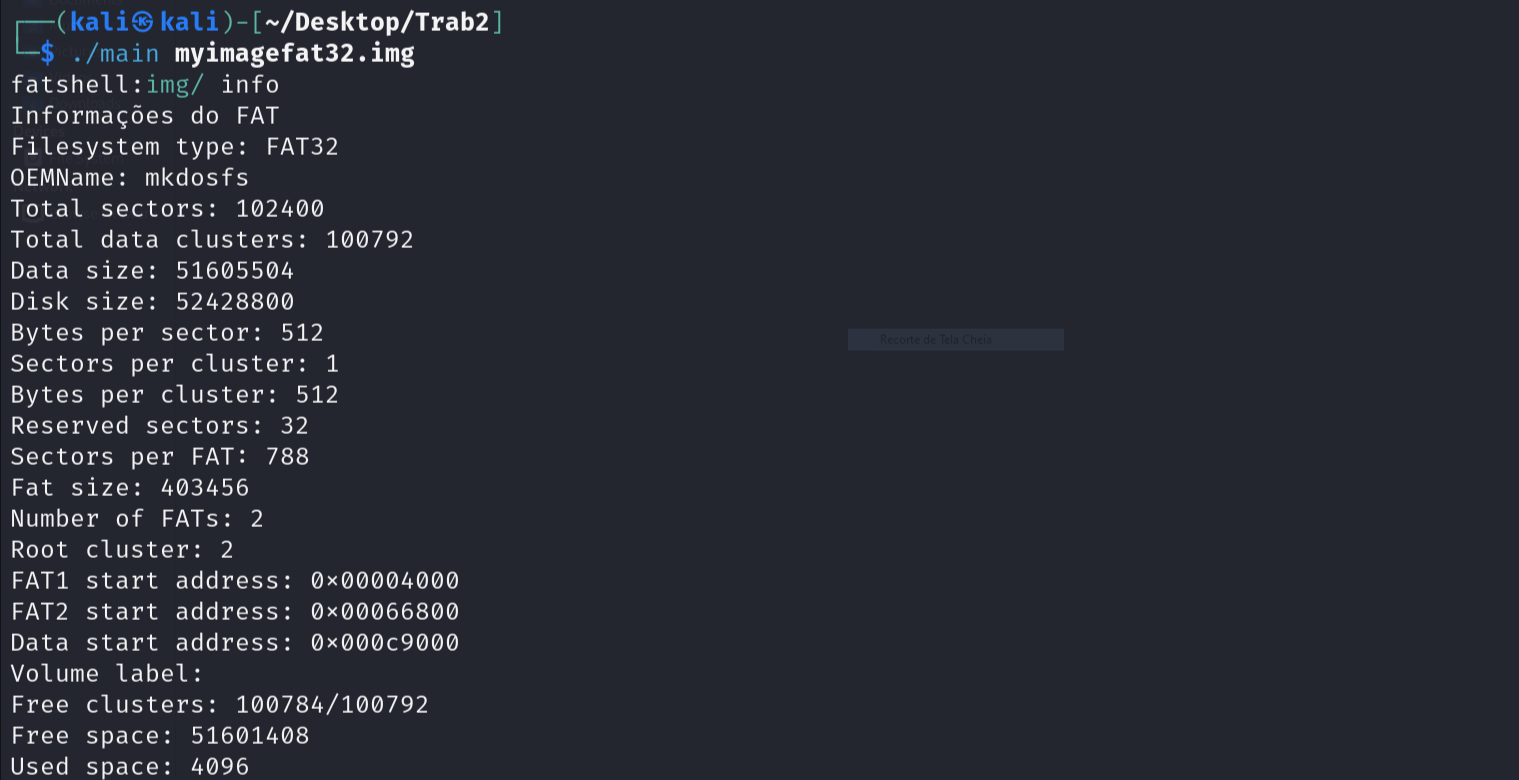
\includegraphics[width=450pt]{0-info.PNG}
    \caption{Saída do comando \texttt{info}}
    \label{fig:info}
\end{figure}

% --------------

\subsection{\texttt{ls}}
\label{subsec:ls}
Comando: \$ \texttt{ls [caminho]} 

O comando \texttt{ls} lista os arquivos e diretórios do caminho atual ou do caminho descrito no primeiro parâmetro dele, a sua saída executada no caminho atual pode ser verificada na Figura~\ref{fig:ls}.

\begin{figure}[H]
    \centering
    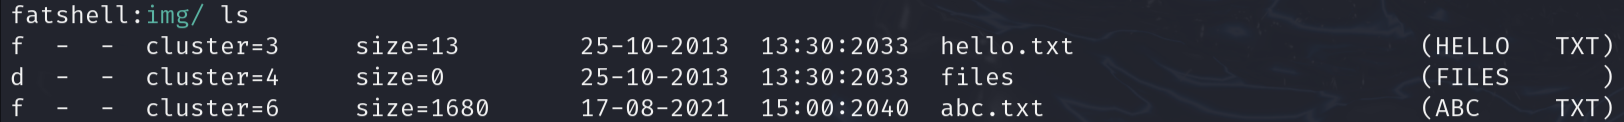
\includegraphics[width=450pt]{figuras/resultados/1-ls.PNG}
    \caption{Saída do comando \texttt{ls} executado no caminho atual}
    \label{fig:ls}
\end{figure}

% --------------

\subsection{\texttt{cluster}}
\label{subsec:cluster}
Comando: \$ \texttt{cluster <número do cluster>}

O comando \texttt{cluster} exibe o conteúdo de um \textit{cluster} em específico, exemplo de uso na Figura~\ref{fig:cluester}.

\begin{figure}[H]
    \centering
    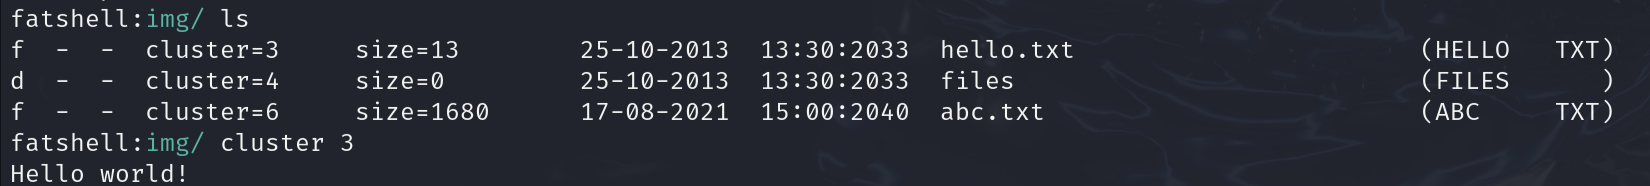
\includegraphics[width=450pt]{figuras/resultados/2-cluster.PNG}
    \caption{Saída do comando \texttt{cluster}}
    \label{fig:cluester}
\end{figure}

% --------------

\subsection{\texttt{cp}}
\label{subsec:cp}
Comando: \$ \texttt{cp <origem> <destino>}  

O comando \texttt{cp} realiza a cópia de um arquivo do caminho de origem para o caminho de destino, podendo efetuar a cópia entre o sistema da imagem e o sistema de arquivo do host sistemas de arquivos ou no próprio sistema da imagem. A cópia de um arquivo externo para o FAT32 pode ser verificada na Figura~\ref{fig:cp-externo-interno-1} e seu resultado na Figura~\ref{fig:cp-externo-interno-2}.

\begin{figure}[H]
    \centering
    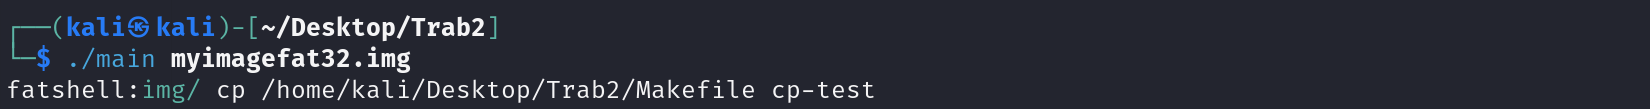
\includegraphics[width=450pt]{figuras/resultados/3.1-cp-externo-interno.PNG}
    \caption{Execução do comando \texttt{cp} para copiar arquivo externo para o FAT32}
    \label{fig:cp-externo-interno-1}
\end{figure}

\begin{figure}[H]
    \centering
    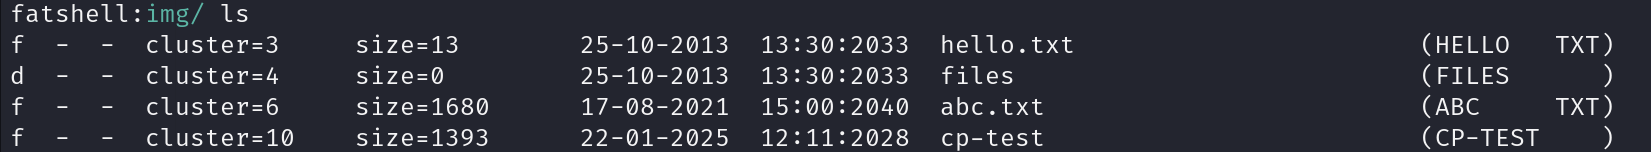
\includegraphics[width=450pt]{figuras/resultados/3.2-cp-externo-interno.PNG}
    \caption{Resultado da cópia do arquivo externo}
    \label{fig:cp-externo-interno-2}
\end{figure}

A cópia de um arquivo para o próprio FAT32 pode ser verificada na Figura~\ref{fig:cp-interno-attr}.

\begin{figure}[H]
    \centering
    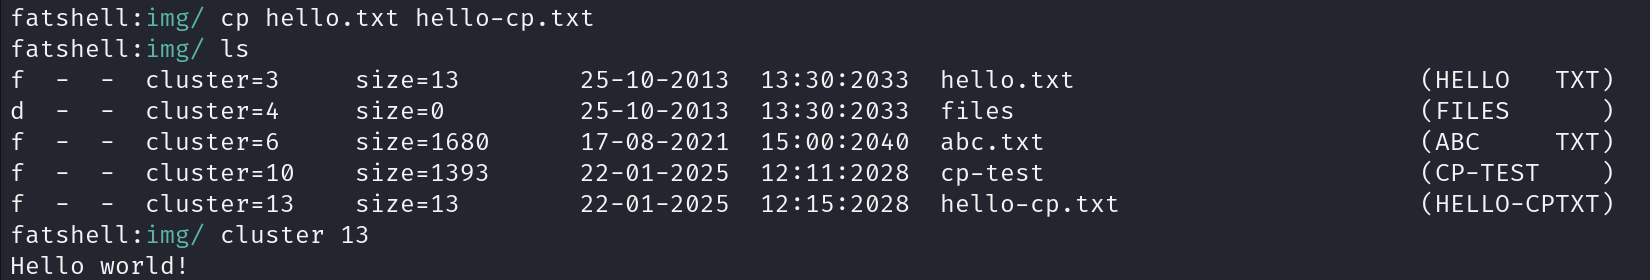
\includegraphics[width=450pt]{figuras/resultados/5-cp-interno-attr.PNG}
    \caption{Execução e resultado do comando \texttt{cp}, utilizado no próprio FAT32}
    \label{fig:cp-interno-attr}
\end{figure}

A cópia do arquivo residente no FAT32 para o sistema de arquivos externo pode ser verificada na Figura~\ref{fig:cp-interno-externo-1} e o seu resultado na Figura~\ref{fig:cp-interno-externo-2}.

\begin{figure}[H]
    \centering
    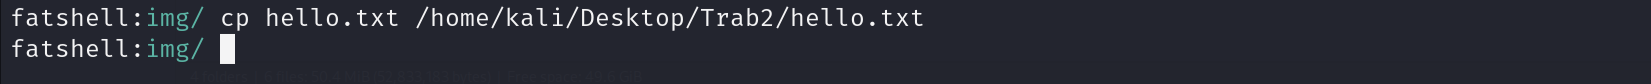
\includegraphics[width=450pt]{figuras/resultados/6-cp-interno-externo.PNG}
    \caption{Execução do comando \texttt{cp} realizando a cópia de um arquivo interno para o sistema de arquivos externo}
    \label{fig:cp-interno-externo-1}
\end{figure}

\begin{figure}[H]
    \centering
    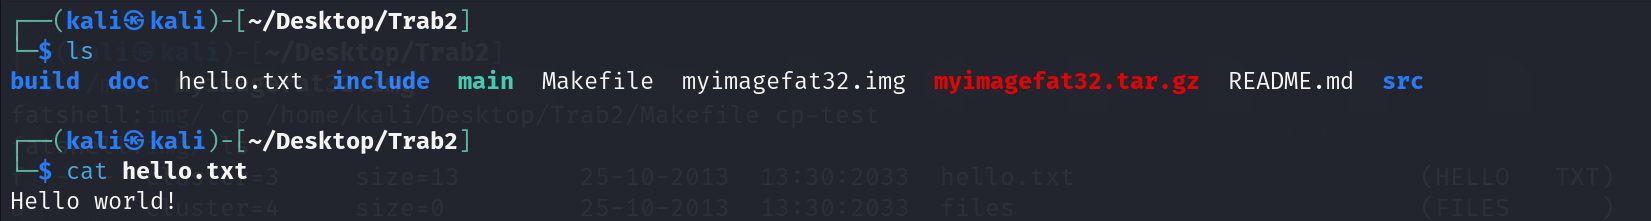
\includegraphics[width=450pt]{figuras/resultados/7-cp-arquivo-externo-resultado.PNG}
    \caption{Resultado no sistema de arquivos internos após cópia de arquivo resistente no FAT32}
    \label{fig:cp-interno-externo-2}
\end{figure}

% --------------

\subsection{\texttt{attr}}
\label{subsec:attr}
Comando: \$ \texttt{attr <diretório | arquivo> }

O comando \texttt{attr} exibe os atributos de um arquivo ou diretório, a Figura~\ref{fig:attr} mostra a saída deste comando.

\begin{figure}[H]
    \centering
    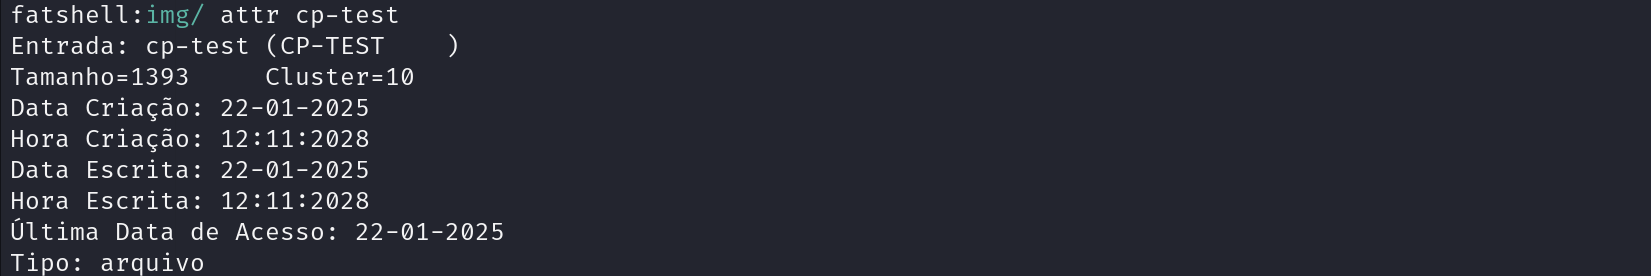
\includegraphics[width=450pt]{figuras/resultados/4-attr.PNG}
    \caption{Exemplo de saída para o comando \texttt{attr} utilizado em um arquivo}
    \label{fig:attr}
\end{figure}

% --------------

\subsection{\texttt{touch}}
\label{subsec:touch}
Comando: \$ \texttt{touch <nome>} 

O comando \texttt{touch} cria um arquivo sem conteúdo, a Figura~\ref{fig:touch} mostra a execução deste comando.

\begin{figure}[h!]
    \centering
    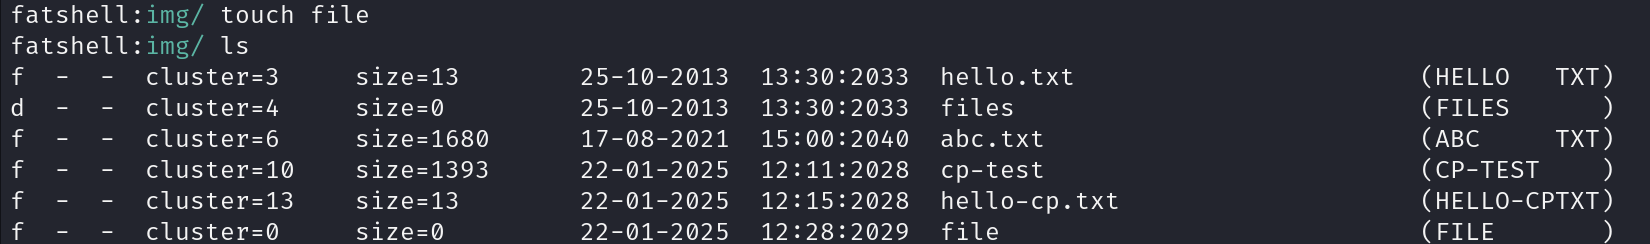
\includegraphics[width=450pt]{figuras/resultados/8-touch.PNG}
    \caption{Exemplo de uso do comando \texttt{touch}}
    \label{fig:touch}
\end{figure}

% --------------

\subsection{\texttt{mkdir}}
\label{subsec:mkdir}
Comando: \$ \texttt{mkdir <nome>}

O comando \texttt{mkdir} cria um diretório vazio, um exemplo da sua utilização pode ser analisado na Figura~\ref{fig:mkdir}.

\begin{figure}[H]
    \centering
    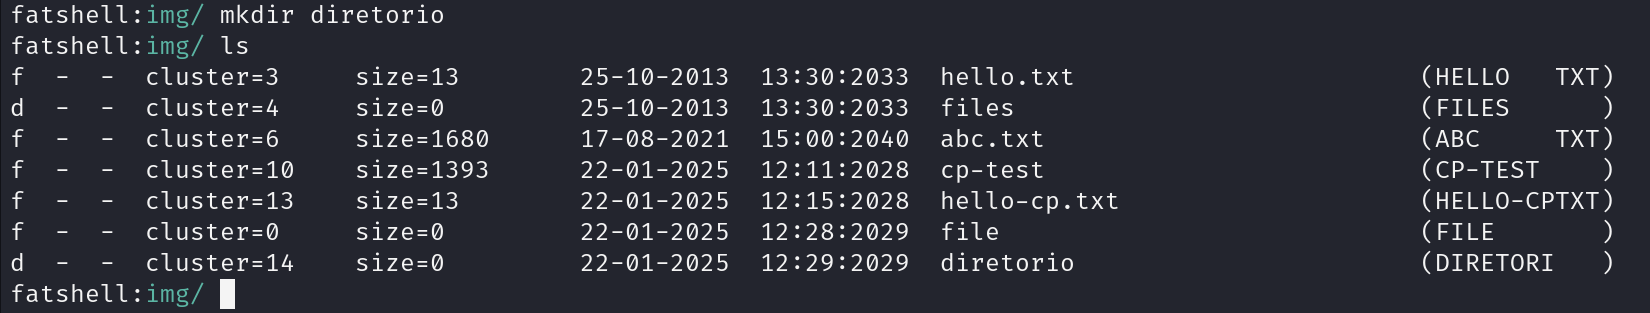
\includegraphics[width=450pt]{figuras/resultados/9-mkdir.PNG}
    \caption{Exemplo de uso do comando \texttt{mkdir}}
    \label{fig:mkdir}
\end{figure}

% --------------

\subsection{\texttt{cd}}
\label{subsec:cd}
Comando: \$ \texttt{cd <destino>}

O comando \texttt{cd} possibilita navegar entre os diretórios, um exemplo da sua utilização pode ser analisado na Figura~\ref{fig:cd}.
 
\begin{figure}[H]
    \centering
    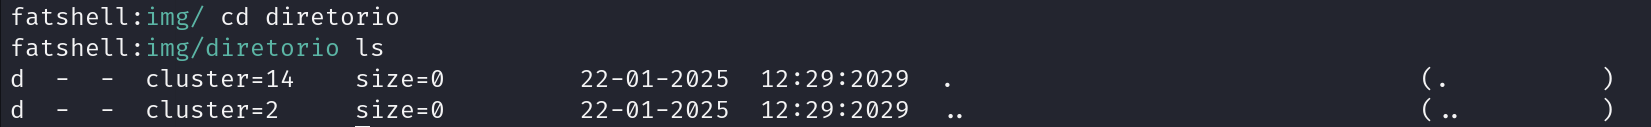
\includegraphics[width=450pt]{figuras/resultados/10-cd.PNG}
    \caption{Exemplo de utilização do comando \texttt{cd}}
    \label{fig:cd}
\end{figure}

% --------------

\subsection{\texttt{rename}}
\label{subsec:rename}
Comando: \$ \texttt{rename <arquivo alvo> <arquivo com novo nome>}

O comando \texttt{rename} altera o nome de um arquivo específico, um exemplo da sua utilização pode ser analisado na Figura~\ref{fig:rename}.

\begin{figure}[H]
    \centering
    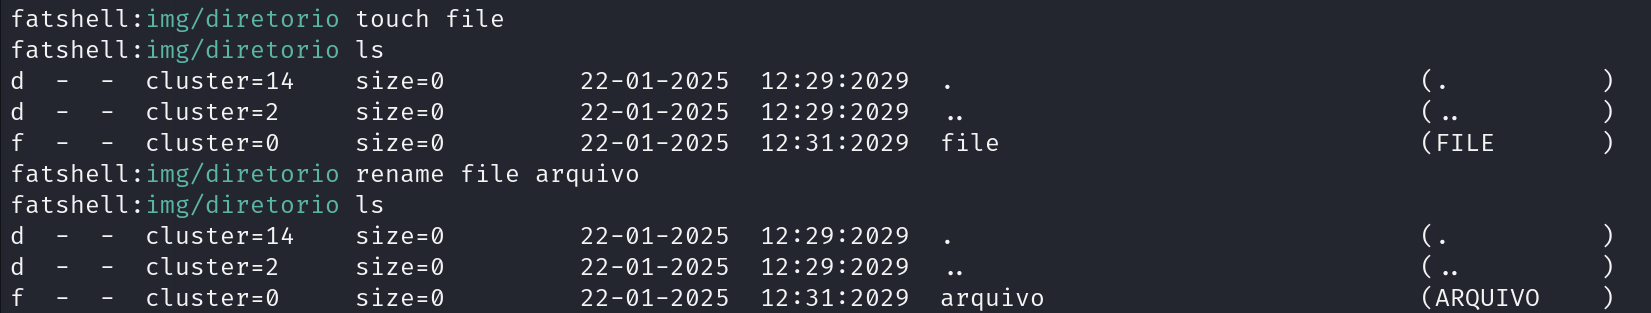
\includegraphics[width=450pt]{figuras/resultados/11-rename.PNG}
    \caption{Exemplo de utilização do comando \texttt{rename}}
    \label{fig:rename}
\end{figure}

% --------------

\subsection{\texttt{mv}}
\label{subsec:mv}
Comando: \$ \texttt{mv <origem> <destino>}

O comando \texttt{mv} move arquivos para um destino específico, assim como o comando \texttt{cp} também pode ser usado para interagir com o sistema de arquivo original do sistema operacional, um exemplo da sua utilização movendo um arquivo do sistema de arquivos externo para o FAT32, pode ser analisado na Figura~\ref{subsec:mv}.

\begin{figure}[H]
    \centering
    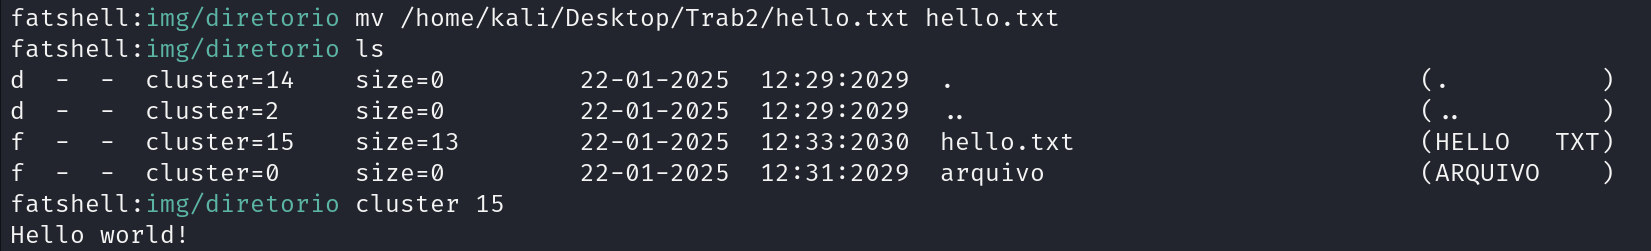
\includegraphics[width=450pt]{figuras/resultados/12-mv-externo-iterno.PNG}
    \caption{Exemplo do comando \texttt{mv} movendo arquivo externo para o FAT32}
    \label{fig:mv-externo-interno}
\end{figure}

O exemplo de mover um arquivo do FAT32 para o sistema de arquivos externo pode ser analisado na Figura~\ref{fig:mv-interno-externo} e sua validação na Figura~\ref{fig:mv-externo-validacao}.

\begin{figure}[H]
    \centering
    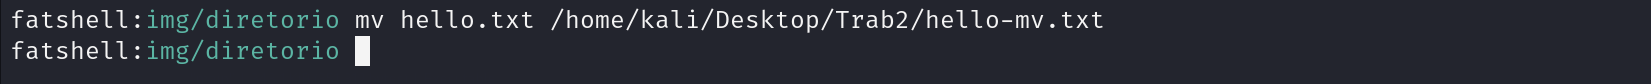
\includegraphics[width=450pt]{figuras/resultados/13-mv-interno-externo.PNG}
    \caption{Exemplo do comando \texttt{mv} movendo um arquivo do FAT32 para o sistema de arquivos externo}
    \label{fig:mv-interno-externo}
\end{figure}

\begin{figure}[H]
    \centering
    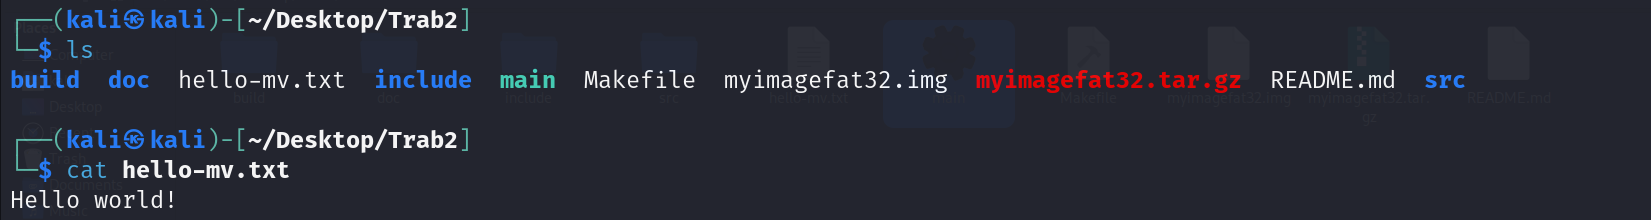
\includegraphics[width=450pt]{figuras/resultados/14-mv-externo-validacao.PNG}
    \caption{Resultado do comando \texttt{mv} movendo um arquivo do FAT32 para o sistema de arquivos externo}
    \label{fig:mv-externo-validacao}
\end{figure}

O exemplo de mover um arquivo interno para o próprio FAT32, pode ser verificado na Figura~\ref{fig:mv-interno}.

\begin{figure}[H]
    \centering
    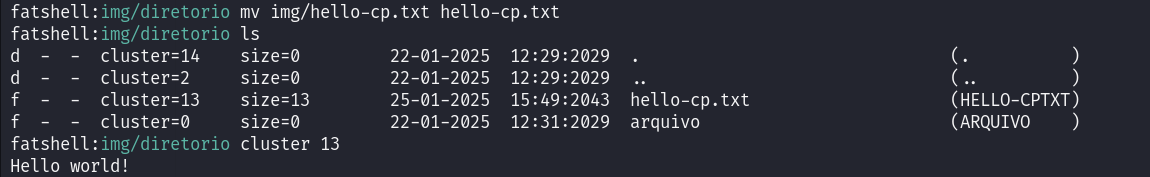
\includegraphics[width=450pt]{figuras/resultados/18-mv-interno-interno.PNG}
    \caption{Exemplo do comando \texttt{mv} movendo arquivo internamente no FAT32}
    \label{fig:mv-interno}
\end{figure}

% --------------

\subsection{\texttt{rm}}
\label{subsec:rm}
Comando: \$ \texttt{rm <arquivo>}

O comando \texttt{rm} remove um arquivo em específico do sistema de arquivos, um exemplo para sua utilização pode ser encontrado na Figura~\ref{fig:rm}.

\begin{figure}[H]
    \centering
    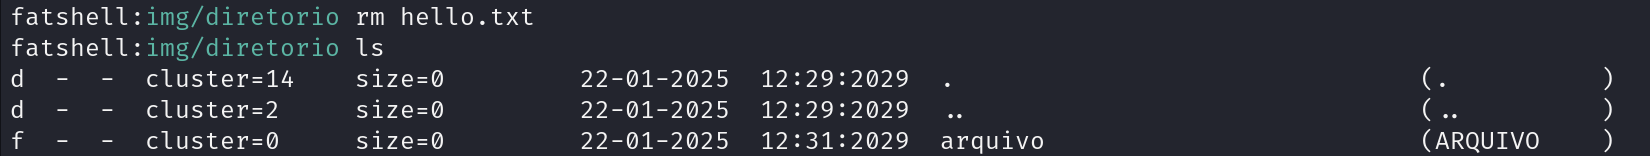
\includegraphics[width=450pt]{figuras/resultados/16-rm.PNG}
    \caption{Exemplo da utilização do comando \texttt{rm}}
    \label{fig:rm}
\end{figure}

% --------------

\subsection{\texttt{rmdir}}
\label{subsec:rmdir}
Comando: \$ \texttt{rmdir <diretório>}

O comando \texttt{rmdir} remove um diretório específico caso ele esteja vazio, um exemplo da sua utilização pode ser encontrado na Figura~\ref{fig:rmdir}.

\begin{figure}[H]
    \centering
    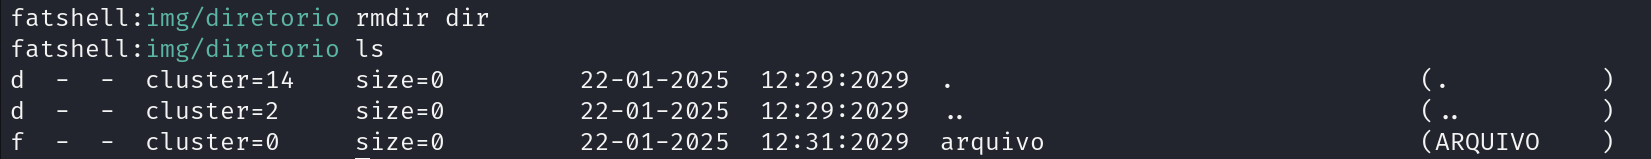
\includegraphics[width=450pt]{figuras/resultados/17-rmdir.PNG}
    \caption{Exemplo da utilização do comando \texttt{rmdir}}
    \label{fig:rmdir}
\end{figure}

% --------------

\subsection{\texttt{pwd}}
\label{subsec:pwd}
Comando: \$ \texttt{pwd}

O comando \texttt{pwd} exibe o caminho absoluto atual, um exemplo da sua saída pode ser encontrado na Figura~\ref{fig:pwd}.

\begin{figure}[H]
    \centering
    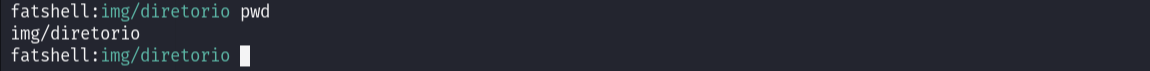
\includegraphics[width=450pt]{figuras/resultados/19-pwd.PNG}
    \caption{Exemplo da saída do comando \texttt{pwd}}
    \label{fig:pwd}
\end{figure}

% --------------

\section{Conclusões}
\label{sec:conclusoes}
A implementação do sistema de arquivos FAT32 permitiu consolidar conceitos teóricos sobre a organização e implementação de um sistema de arquivos, em especial o FAT32, destacando a sua organização de dados em disco, gerenciamento de metadados e alocação de \textit{clusters}. A estrutura modular do código, dividida em componentes como tabela FAT, entradas de diretório e manipulação de imagens de disco, facilitou a manutenção e o teste individual de cada funcionalidade. O \textit{shell} desenvolvido provou ser eficaz na interação com o sistema, executando comandos complexos como cópia entre sistemas de arquivos externos e internos, movimentação de arquivos e renomeação. Os principais desafios durante a implementação do sistema foi a manipulação de nomes longos e a garantia de integridade do sistema todo. Ainda assim, acreditamos que o resultado foi positivo, tanto para o nosso aprendizado quanto para o êxito do projeto em si.

% ----------------------------------------------------------
% ELEMENTOS PÓS-TEXTUAIS
% ----------------------------------------------------------
\postextual
% ----------------------------------------------------------
% Referências bibliográficas
% ----------------------------------------------------------
\renewcommand{\bibsection}{%
\section{\bibname}
\bibmark
%\ifnobibintoc\else
%\phantomsection
%\addcontentsline{toc}{section}{\bibname}
%\fi
\prebibhook}

\bibliography{abntex2-modelo-references}

\end{document}

